\documentclass[12pt]{article}
\usepackage{times}
\usepackage{geometry}
\usepackage[english]{babel}
\usepackage[utf8]{inputenc}
\usepackage{fancyhdr}
\usepackage{graphicx}
\usepackage{titlesec}
\usepackage{biblatex}
\usepackage{minted}
\usepackage{xcolor} % to access the named colour LightGray
\definecolor{LightGray}{gray}{0.9}

\addbibresource{References.bib}


\setlength{\headheight}{15.2pt}
\setcounter{secnumdepth}{3}
\rfoot{Pg: \thepage}

\geometry{
   a4paper,
   left = 25mm,
   top = 20mm,
}
\begin{document}
\thispagestyle{empty}

\section*{}
 {\LARGE\makebox[\textwidth]{\textbf{KATHMANDU UNIVERSITY}}}

\centerline{Department of Computer Science and Engineering}
\centerline{Dhulikhel,Kavre}
\begin{figure}[h]
    \centerline{
\includegraphics[width=50.546mm,height=50.546mm]{KU_Logo.png}}
\end{figure}

\centerline{\textbf{A Lab Report}}
\centerline{on}
\centerline{\underline{\textbf{"Lab 3"}}}

\vspace*{12mm}

\centerline{\textbf{[Code No. : COMP 342]}}
\centerline{(For partial fulfillment of 3rd Year/ 1st Semester in Computer Science)}

\vspace*{20mm}

\centerline{\textbf{Submitted by}}
\centerline{\textbf{Aayush Pokharel (Roll No. 43)}}


\vspace*{26mm}


\centerline{\textbf{Submitted to}}
\centerline{\textbf{Dhiraj Shrestha}}
\centerline{\textbf{Dept of Computer Science and Engineering}}

\vspace*{20mm}

\centerline{\textbf{Submission Date: 18th December, 2022}}



\clearpage
\thispagestyle{empty}


\section*{Abstract}
The report is drafted to meet the prerequisites to partially fulfill the COMP 342 course offered by the
Department of Computer Science and Engineering at Kathmandu University. This project is designed
to expand the knowledge of OpenGL and implement of Eclipse and Circle Drawing Algorithm that we learned in class.
\\\\
\textbf{Keywords:} OpenGL

\clearpage
\thispagestyle{empty}
\tableofcontents

\clearpage
\thispagestyle{empty}
\listoffigures

\clearpage
\pagenumbering{arabic}
\section{CHAPTER 1: INTRODUCTION}

\subsection{Environment}
The lab progam was written using the python programming language and OpenGL rendering Library. To write the program a virtual environment is
created and set of libraries is downloaded for the local virtual environment. Then the python interperter runs under this virtual environment
to run the program

\subsection{OpenGL}
The OpenGL rendering library is written in C programming language and a wrapper library called PyOpenGL is available under BSD-style Open-Source licence which translates the
API calls of OpenGL to Python programming.

\subsection{PyGame}
The PyGame is a cross-platform set of Python modules for game development. Despite being a complete package that can handle all the rendering in a highly abstracted manner, the
limitation of only using OpenGL for the lab work required that it only be used as windowing library under a double buffer system and all the relevant rendering process be done by PyOpenGL itself.

\section{CHAPTER 2: ALGORITHM}
We have read about two different Line Drawing Algorithms in our class. They are as folows:
\begin{itemize}
    \item MidPoint Circle Drawing Algorithm
    \item MidPoint Eclipse Drawing Algorithm
\end{itemize}
\clearpage
\section{CHAPTER 3: CODE}

\subsection{MidPoint Circle Drawing Algorithm}
This is the code for the MidPoint Circle Drawing Algorithm.
\begin{minted}[
    frame=lines,
    framesep=2mm,
    baselinestretch=1.2,
    bgcolor=LightGray,
    fontsize=\footnotesize,
    linenos
    ]{python}
import ctypes
import numpy as np
from OpenGL.GL import *
from OpenGL.GLU import *
import pygame as pg
from pygame.locals import *

# Define Shaders
vertexShader = """
attribute vec2 position;
void main()
{
  gl_Position = vec4(position, 0.0, 1.0);
}
"""

fragmentShader = """
void main()
{
  gl_FragColor = vec4(0.0,1.0,0.0,1.0);
}
"""


def normalize(xList, yList, resolution):
    xList = [x / resolution for x in xList]
    yList = [y / resolution for y in yList]

    coordinateList = np.zeros((len(xList), 2))
    i = 0
    for _ in xList:
        coordinateList[i] = [xList[i], yList[i]]
        i += 1
    return coordinateList


def midpoint_circle(x_center, y_center, r, res):
    x = r
    y = 0
    # Printing the initial point the
    # axes after translation
    x_coordinates = np.array([])
    y_coordinates = np.array([])

    x_coordinates = np.append(x_coordinates, x + x_center)
    y_coordinates = np.append(y_coordinates, y + y_center)
    # When radius is zero only a single
    # point be printed
    if r > 0:
        x_coordinates = np.append(x_coordinates, x + x_center)
        x_coordinates = np.append(x_coordinates, y + x_center)
        x_coordinates = np.append(x_coordinates, -y + x_center)
        y_coordinates = np.append(y_coordinates, -y + y_center)
        y_coordinates = np.append(y_coordinates, x + y_center)
        y_coordinates = np.append(y_coordinates, x + y_center)

    P = 1 - r

    while x > y:

        y += 1

        if P <= 0:
            P = P + 2 * y + 1

        else:
            x -= 1
            P = P + 2 * y - 2 * x + 1

        if x < y:
            break

        x_coordinates = np.append(x_coordinates, x + x_center)
        x_coordinates = np.append(x_coordinates, -x + x_center)
        x_coordinates = np.append(x_coordinates, x + x_center)
        x_coordinates = np.append(x_coordinates, -x + x_center)
        y_coordinates = np.append(y_coordinates, y + y_center)
        y_coordinates = np.append(y_coordinates, y + y_center)
        y_coordinates = np.append(y_coordinates, -y + y_center)
        y_coordinates = np.append(y_coordinates, -y + y_center)

        if x != y:
            x_coordinates = np.append(
                x_coordinates,
                y + x_center,
            )
            x_coordinates = np.append(x_coordinates, -y + x_center)
            x_coordinates = np.append(x_coordinates, y + x_center)
            x_coordinates = np.append(x_coordinates, -y + x_center)
            y_coordinates = np.append(y_coordinates, x + y_center)
            y_coordinates = np.append(y_coordinates, x + y_center)
            y_coordinates = np.append(y_coordinates, -x + y_center)
            y_coordinates = np.append(y_coordinates, -x + y_center)

    return normalize(x_coordinates, y_coordinates, res)


tempData = midpoint_circle(0, 0, 500, 1000)
data = np.zeros(int(len(tempData)), [("position", np.float32, 2)])
data["position"] = tempData


def compileShader(source, type):
    shader = glCreateShader(type)
    glShaderSource(shader, source)

    glCompileShader(shader)
    if not glGetShaderiv(shader, GL_COMPILE_STATUS):
        error = glGetShaderInfoLog(shader).decode()
        print(error)
        raise RuntimeError(f"{source} shader compilation error")
    return shader


def createProgram(vertex, fragment):
    program = glCreateProgram()
    glAttachShader(program, vertex)
    glAttachShader(program, fragment)

    glLinkProgram(program)
    if not glGetProgramiv(program, GL_LINK_STATUS):
        print(glGetProgramInfoLog(program))
        raise RuntimeError("Error Linking program")

    glDetachShader(program, vertex)
    glDetachShader(program, fragment)

    return program


def main():
    running = True
    while running:
        width, height = 800, 800
        pg.init()
        pg.display.set_mode(
            (width, height), DOUBLEBUF | OPENGL | GL_RGBA)
        pg.display.set_caption(
            "Midpoint Circle - Lab 3 | Aayush Pokharel")
        glViewport(0, 0, width, height)
        # here inti()
        glClear(GL_COLOR_BUFFER_BIT)
        glClearColor(0.0, 0.0, 0.0, 1.0)
        glLoadIdentity()

        program = createProgram(
            compileShader(vertexShader, GL_VERTEX_SHADER),
            compileShader(fragmentShader, GL_FRAGMENT_SHADER),
        )

        glUseProgram(program)

        buffer = glGenBuffers(1)
        glBindBuffer(GL_ARRAY_BUFFER, buffer)

        stride = data.strides[0]
        offset = ctypes.c_void_p(0)
        loc = glGetAttribLocation(program, "position")
        glEnableVertexAttribArray(loc)
        glBindBuffer(GL_ARRAY_BUFFER, buffer)
        glVertexAttribPointer(loc, 3, GL_FLOAT, False, stride, offset)

        glBufferData(GL_ARRAY_BUFFER, data.nbytes, data, GL_STATIC_DRAW)
        glDrawArrays(GL_POINTS, 0, len(data))
        pg.display.flip()

        for event in pg.event.get():
            if event.type == pg.QUIT:
                running = False


if __name__ == "__main__":
    main()
\end{minted}
\clearpage
\subsection{MidPoint Eclipse Drawing Algorithm}
This is the code for the MidPoint Eclipse Drawing Algorithm.
\begin{minted}[
    frame=lines,
    framesep=2mm,
    baselinestretch=1.2,
    bgcolor=LightGray,
    fontsize=\footnotesize,
    linenos
    ]{python}
import ctypes
import numpy as np
from OpenGL.GL import *
from OpenGL.GLU import *
import pygame as pg
from pygame.locals import *

# Define Shaders
vertexShader = """
attribute vec2 position;
void main()
{
  gl_Position = vec4(position, 0.0, 1.0);
}
"""

fragmentShader = """
void main()
{
  gl_FragColor = vec4(1.0,0.0,0.0,1.0);
}
"""


def normalize(xList, yList, resolution):
    xList = [x / resolution for x in xList]
    yList = [y / resolution for y in yList]

    coordinateList = np.zeros((len(xList), 2))
    i = 0
    for _ in xList:
        coordinateList[i] = [xList[i], yList[i]]
        i += 1
    return coordinateList


def midpoint_ellipse(rx, ry, xc, yc, res):
    x = 0
    y = ry

    x_coordinates = np.array([])
    y_coordinates = np.array([])

    # Initial decision parameter of region 1
    d1 = (ry * ry) - (rx * rx * ry) + (0.25 * rx * rx)
    dx = 2 * ry * ry * x
    dy = 2 * rx * rx * y
    # For region 1
    while dx < dy:
        x_coordinates = np.append(x_coordinates, x + xc)
        x_coordinates = np.append(x_coordinates, -x + xc)
        x_coordinates = np.append(x_coordinates, x + xc)
        x_coordinates = np.append(x_coordinates, -x + xc)
        y_coordinates = np.append(y_coordinates, y + yc)
        y_coordinates = np.append(y_coordinates, y + yc)
        y_coordinates = np.append(y_coordinates, -y + yc)
        y_coordinates = np.append(y_coordinates, -y + yc)

        if d1 < 0:
            x += 1
            dx = dx + (2 * ry * ry)
            d1 = d1 + dx + (ry * ry)
        else:
            x += 1
            y -= 1
            dx = dx + (2 * ry * ry)
            dy = dy - (2 * rx * rx)
            d1 = d1 + dx - dy + (ry * ry)

    # Decision parameter of region 2
    d2 = (
        ((ry * ry) * ((x + 0.5) * (x + 0.5)))
        + ((rx * rx) * ((y - 1) * (y - 1)))
        - (rx * rx * ry * ry)
    )

    # Plotting points of region 2
    while y >= 0:
        x_coordinates = np.append(x_coordinates, x + xc)
        x_coordinates = np.append(x_coordinates, -x + xc)
        x_coordinates = np.append(x_coordinates, x + xc)
        x_coordinates = np.append(x_coordinates, -x + xc)
        y_coordinates = np.append(y_coordinates, y + yc)
        y_coordinates = np.append(y_coordinates, y + yc)
        y_coordinates = np.append(y_coordinates, -y + yc)
        y_coordinates = np.append(y_coordinates, -y + yc)

        if d2 > 0:
            y -= 1
            dy = dy - (2 * rx * rx)
            d2 = d2 + (rx * rx) - dy
        else:
            y -= 1
            x += 1
            dx = dx + (2 * ry * ry)
            dy = dy - (2 * rx * rx)
            d2 = d2 + dx - dy + (rx * rx)

    return normalize(x_coordinates, y_coordinates, res)


tempData = midpoint_ellipse(800, 400, 0, 0, 1000)
data = np.zeros(int(len(tempData)), [("position", np.float32, 2)])
data["position"] = tempData


def compileShader(source, type):
    shader = glCreateShader(type)
    glShaderSource(shader, source)

    glCompileShader(shader)
    if not glGetShaderiv(shader, GL_COMPILE_STATUS):
        error = glGetShaderInfoLog(shader).decode()
        print(error)
        raise RuntimeError(f"{source} shader compilation error")
    return shader


def createProgram(vertex, fragment):
    program = glCreateProgram()
    glAttachShader(program, vertex)
    glAttachShader(program, fragment)

    glLinkProgram(program)
    if not glGetProgramiv(program, GL_LINK_STATUS):
        print(glGetProgramInfoLog(program))
        raise RuntimeError("Error Linking program")

    glDetachShader(program, vertex)
    glDetachShader(program, fragment)

    return program


def main():
    running = True
    while running:
        width, height = 800, 800
        pg.init()
        pg.display.set_mode((width, height),
        DOUBLEBUF | OPENGL | GL_RGBA)
        pg.display.set_caption(
            "Midpoint Ellipse - Lab 3 | Aayush Pokharel")
        glViewport(0, 0, width, height)
        # here inti()
        glClear(GL_COLOR_BUFFER_BIT)
        glClearColor(0.0, 0.0, 0.0, 1.0)
        glLoadIdentity()

        program = createProgram(
            compileShader(vertexShader, GL_VERTEX_SHADER),
            compileShader(fragmentShader, GL_FRAGMENT_SHADER),
        )

        glUseProgram(program)

        buffer = glGenBuffers(1)
        glBindBuffer(GL_ARRAY_BUFFER, buffer)

        stride = data.strides[0]
        offset = ctypes.c_void_p(0)
        loc = glGetAttribLocation(program, "position")
        glEnableVertexAttribArray(loc)
        glBindBuffer(GL_ARRAY_BUFFER, buffer)
        glVertexAttribPointer(loc, 3, GL_FLOAT, False, stride, offset)

        glBufferData(GL_ARRAY_BUFFER, data.nbytes, data, GL_STATIC_DRAW)
        glDrawArrays(GL_POINTS, 0, len(data))
        pg.display.flip()

        for event in pg.event.get():
            if event.type == pg.QUIT:
                running = False


if __name__ == "__main__":
    main()

\end{minted}


\clearpage
\section{CHAPTER 3: SCREENSHOTS}
This is the screenshot of the executed program for MidPoint Circle Drawing Algorithm.
\begin{figure}[h]
    \centerline{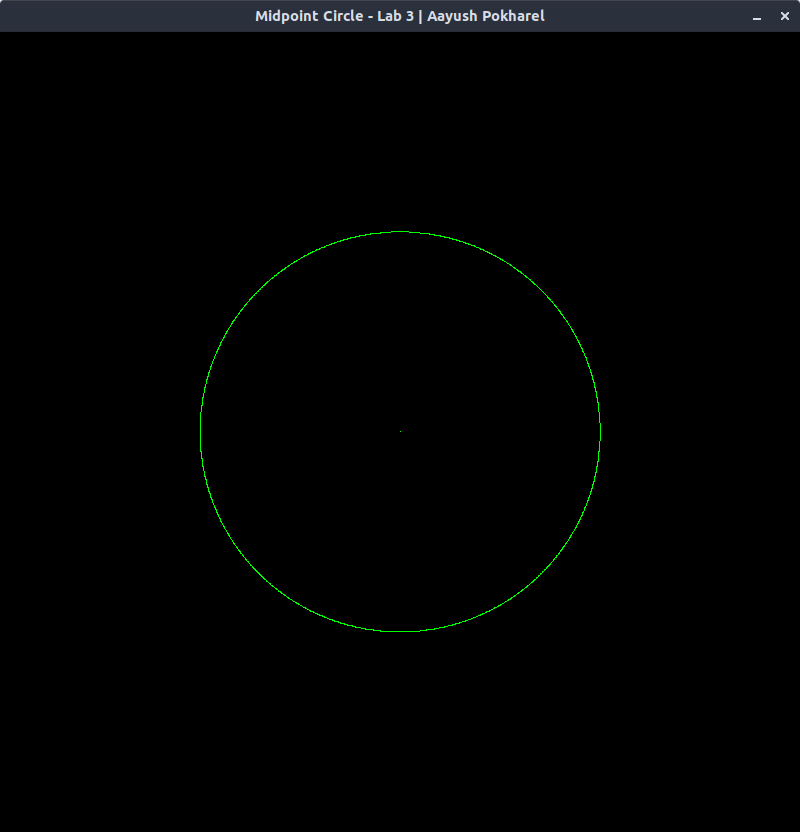
\includegraphics[height=100mm]{MidPointCircle.png}}
    \caption{MidPoint Circle Drawing Algorithm}
    \label{fig}
\end{figure}
\clearpage
This is the screenshot of the executed program for MidPoint Ellipse Drawing Algorithm.
\begin{figure}[ h ]
    \centerline{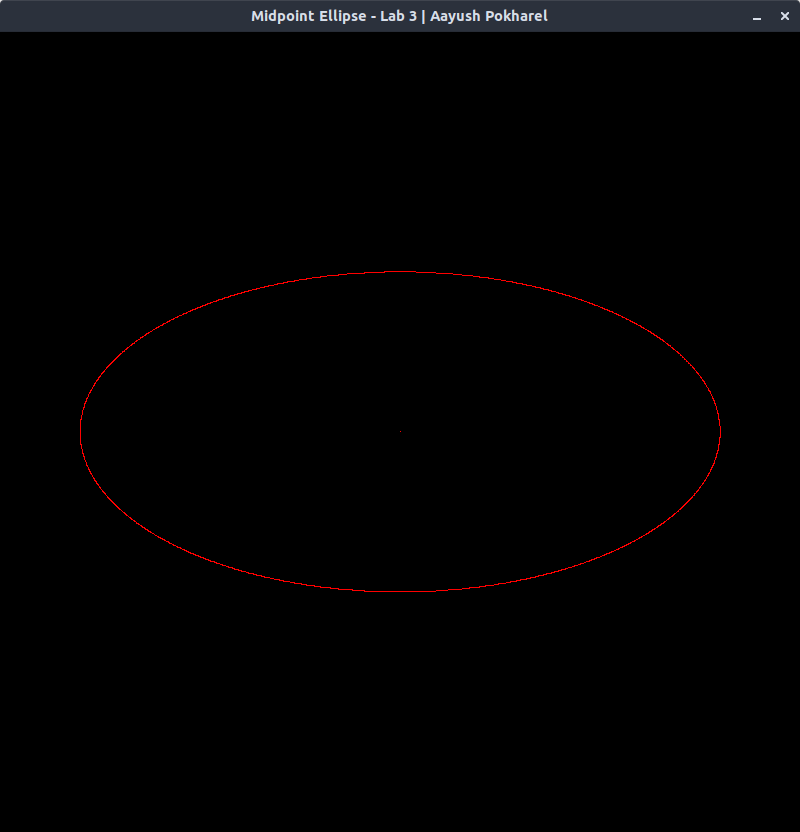
\includegraphics[height=100mm]{MidPointEllipse.png}}
    \caption{MidPoint Ellipse Drawing Algorithm}
    \label{fig}
\end{figure}

\section{CHAPTER 4: CONCLUSION}
In the nutshell, the lab was implement using the programmable shader pipeline of OpenGL. The points were calculated and provided to the rendering pipeline to
bind and display in the screen.
\clearpage
\thispagestyle{empty}
\printbibliography

\end{document}
